% !TEX root = set_recommendation.tex
\section{Introduction}
\label{sec:introduction}
Item attributes provide valuable side information for recommender systems.
\cref{fig:motivating-example} shows an example dataset from a hypothetical diet
tracking app. In this data, $5$ users have eaten meals with various foods or
attributes. The goal is to build a recommender system that suggests meals that
users would enjoy. Leveraging the information about item attributes in
\cref{fig:motivating-example} should improve recommendation performance. For
instance, User 1 may be a pescatarian since they did not log the two meals
containing meat; User 4 is omnivorous. User 3 seems to prefer salads, whereas
User 4 prefers fast foods such as tacos or pizza. These are all observations
made by inspecting the attributes of each meal.

\begin{table*}
    \begin{center}
    \begin{tabular}{@{}lccccccccc|cccccc@{}}
      & \multicolumn{9}{c}{\bf Attributes (foods)} & \multicolumn{5}{c}{\bf
                                                     Users}\\
      \cmidrule(lr){2-10} \cmidrule(lr){11-15}
      {\bf Items (meals)} & Pizza & Eggs & Taco & Salad & Avocado & Chicken & Sardines & Beer & Coffee & 1 & 2 & 3 & 4 & 5 \\
      Breakfast pizza with coffee & \faCheck & \faCheck & & & & & & & \faCheck & & \faCheck & & \faCheck & \\
      Dinner pizza & \faCheck & & & & & & \faCheck & \faCheck & & \faCheck & & & \faCheck & \\
      Small salad & & & & \faCheck & \faCheck & & \faCheck & & & & & \faCheck & & \faCheck \\
      Big salad & & \faCheck & & \faCheck & \faCheck & \faCheck & & & \faCheck & & & \faCheck & \faCheck & \\
      Taco & & & \faCheck & & \faCheck & \faCheck & & & \faCheck & & & & & \faCheck \\
      Sardine taco & & & \faCheck & & & & \faCheck & & & \faCheck & \faCheck & & \faCheck & \\
      \bottomrule
    \end{tabular}
    \caption{\label{fig:motivating-example}An example of the data we focus on,
      where tagged items are recommended to users based on both the item
      attributes and the items users have consumed in the past. This example
      dataset of meals is made up of meals with different foods (left) and users
      logging which meals they ate (right). The goal is to leverage the
      attributes to recommend items to users.}
    \end{center}
\end{table*}

% \begin{table*}
%     \begin{center}
%     \begin{tabular}{@{}lccccccc|cccccc@{}}
%       & \multicolumn{7}{c}{\bf Attributes (tags)} & \multicolumn{5}{c}{\bf
%                                                      Users}\\
%       \cmidrule(lr){2-8} \cmidrule(lr){9-13}
%       {\bf Items (news articles)} & Politics & Election & Gossip & Security & Technology & Sports & New York & 1 & 2 & 3 & 4 & 5 \\
%       Political scandal & \faCheck & \faCheck & \faCheck & & & & & & & & & \\
%       NYC mayoral election debate & \faCheck & \faCheck & & & & & \faCheck & & & & &  \\
%       Celebrity couple pregnancy & & & \faCheck & & & & & & & & &  \\
%       Voting machine security & & \faCheck & & \faCheck & \faCheck & & & & & & &  \\
%       Border security & \faCheck & \faCheck & & \faCheck & & & & & & & &  \\
%       Immigration reform bill & \faCheck & & & & & & & & & & & \\
%       New iPhone specs & & & &  & \faCheck & & & & & & & \\
%       NYC subway bill & \faCheck & & & & & & \faCheck & & & & &  \\
%       NY Yankees game results & & & & & & \faCheck & \faCheck & & & & &  \\
%       NY Knicks game results & & & & & & \faCheck & \faCheck & & & & &  \\
%       Boston Red Sox game results & & & & & & \faCheck & & & & & &  \\
%       \bottomrule
%     \end{tabular}
%     \caption{\label{fig:motivating-example}An example of the data we focus on,
%       where tagged items are recommended to users based on both the item
%       attributes and the items users have consumed in the past. This example
%       dataset of meals is made up of meals with different foods (left) and users
%       logging which meals they ate (right). The goal is to leverage the
%       attributes to recommend items to users.}
%     \end{center}
% \end{table*}

%%% Local Variables:
%%% mode: latex
%%% TeX-master: "../set_recommendation"
%%% End:


Modeling item attributes in a recommender system is not straightforward. There
are nonlinear relationships between attributes and users. In the meals example,
User 2 enjoys pizza, eggs, coffee, and sardine tacos. But a recommendation that
melds eggs and sardines would not be met with enthusiasm. Furthermore, there are
many types of the same attribute, such as many varieties of pizza. This leads to
millions of unique foods. For a recommender system to scale, it must be able to
handle a large number of item attributes.

In addition to many attributes, there are an even larger number of items. In the
case of meals, we cannot even represent every possible item: any new combination
of foods represents an entirely new meal. Traditional content-based recommender
systems such as content-based matrix factorization
models~\cite{wang2011collaborative,gopalan2014content-based} require parameters
to be learned for every item, and cannot scale to this type of data. In addition
to being unscalable, these models' objective functions are the log-likelihood of
the data or a bound on the log-likelihood. Such objective functions are
well-justified theoretically, but are not tied to the evaluation metrics used to
evaluate recommender systems.
% Meals containing
% only one or two foods, or those ordered at chain restaurants, may be logged by
% many users. But these represent a small proportion of the meals people actually
% eat. Consequently, a long tail of meals are logged by only a single user.

This paper proposes \gls{rfs}, a scalable model for recommending items with
attributes. \gls{rfs} casts the recommendation problem as binary classification.
Given an item and a user, \gls{rfs} treats attributes as features classifies
whether or not the item is likely to be consumed by the user. \gls{rfs} learns
embeddings for each user and attribute; each item is represented as the mean of
its attribute embeddings. To scale to large data, \gls{rfs} is trained using a
stochastic optimization-based negative sampling procedure that randomly samples
items that are unlikely to be consumed.

\gls{rfs} enjoys two benefits from framing the recommendation problem as
classification. First, the \gls{rfs} classification objective function is
directly tied to an evaluation metric, and we show that a classifier with zero
worst-case error achieves maximum recall. Then we describe how a plethora of
deep learning models for classification can be exploited for recommendation; for
example, we parameterize \gls{rfs} with a deep residual network. Ultimately, we
apply existing theory~\cite{zaheer2017deep} for neural networks that operate on
set-valued input to show that \gls{rfs} can approximate principled
recommendation models such as content-based matrix
factorization~\cite{gopalan2014content-based}.

We study \gls{rfs} on two datasets. We consider a dataset of $65$k users
clicking on $637$k papers posted to the arXiv; the attributes of a paper are the
unique words in its abstract. \gls{rfs} outperforms a state-of-the-art
content-based matrix factorization model~\cite{gopalan2014content-based} on this
dataset, and the learned document embeddings capture the structure of
human-labeled topics. Second, we consider a large dataset of $55$k users logging
$16$M meals using the LoseIt! diet tracking app. Again, \gls{rfs} outperforms
other baseline models, and the learned meal embeddings reveal a diverse set of
recommendations that capture the notion of taste.

\gls{rfs} is extremely scalable and is fit with a loss function tied to an
evaluation metric. In addition to outperforming competitors on large datasets,
it is backed by an ability to approximate other models that recommend items with
attributes. \emph{This work demonstrates that if a practitioner aims to perform
  recommendation of items with attributes and measures recommendation
  performance with recall, the best choice of model is a deep classifier such as
  \gls{rfs}.}


% !TEX root = ../set_recommendation.tex
\begin{figure*}[t!]
  \centering
%  \pdfimageresolution=500  
  \includegraphics[width=0.95\textwidth]{fig/arxiv_user_embeddings_tsne.png}
  \caption{\label{fig:arxiv_tsne} \acrlong{rfs} trained on arXiv reading
    behavior clusters researchers by their most frequently-read arXiv category
    (best viewed in color). On this data, \acrlong{rfs} is trained to recommend
    items using their attributes as described in \Cref{sec:experiments_arxiv};
    the set of attributes for a paper is the set of words in the abstract. A
    visualization of the user embeddings in the inner product regression
    function in \Cref{eqn:rankfromsets} yields an interpretable map of science.
    We use the t-SNE algorithm~\citep{maaten2008visualizing} for visualizing the
    high-dimensional embeddings in two dimensions. In this map of science,
    fields of study are related according to patterns in how people read papers
    in neighboring fields. Each marker represents a user embedding; the color
    assigned to a user is determined the user's most-read arXiv category. The
    color assigned to a category is determined by the most-read categories
    across the arXiv, with similar colors assigned to similar fields according
    to the arXiv ontology. For an interactive version of this map, please visit
    anon-url which enables zoom and display of all 143 arXiv category labels to
    explore the relationships between different fields of science.}
\end{figure*}


%%% Local Variables:
%%% mode: latex
%%% TeX-master: "../set_recommendation"
%%% End:

% The rest of this paper is organinized as follows:
% \paragraph{Background}
% \begin{itemize}
%     \item Recommendation with side information
%     \item Negative sampling in recommender systems
%     \item Regression models with set-valued features
% \end{itemize}

% \paragraph{Method}
% \begin{itemize}
%     \item Recommendation as classification
%     \item Embedding users and items
%     \item Learning the parameters through negative sampling
% \end{itemize}

% \paragraph{Results}
% \begin{itemize}
%     \item Metrics (recall@K definition)
%     \item Recommending documents
%     \item Recommending meals
% \end{itemize}

% \paragraph{Discussion}
% \begin{itemize}
%     \item Summarize contribution
%     \item Incorporating additional side information
%     \item Other interesting things?
% \end{itemize}
% % set up the task of recommendation, foreshadow how we will solve it via
% % classification
% Sets of attributes represent many types of items. A user might be associated
% with a photo that has tags, a disease with diagnosis codes, or a playlist of
% songs. Recommendation models for such items use the item attributes to rank
% items for users. Central to building recommendation models is evaluation, and a
% common metric is recall. But existing models such as matrix factorization do not
% have associated theoretical guarantees of improved recall. Currently, models are
% built on a case-by-case basis and adapted to the data at hand, and must be
% painstakingly compared to see which extension leads to improvement of the
% evaluation metric.

% % foreshadow desiderata
% Our goal is to build a recommendation model to rank items from attributes, and
% buttress the model with theoretical guarantees of universal approximation
% (ability to approximate other models) and of improved recommendation performance
% vis-\`a-vis recall.

% % desideratum #1: statistical challenge
% Building models that rank items from sets of attributes must address two
% difficulties arising from the properties of sets. The first difficulty is the
% statistical challenge posed by the large number of possible sets. The number of
% sets of attributes is large; we cannot posit a model with unique parameters for
% every set of attributes. The meal recommendation problem illustrates this
% statistical challenge. \Cref{fig:hist} shows the number of meals in data from a
% food tracking app. Even in this small fraction of the data, there are over ten
% million unique meals. In building a recommendation model to rank meals based on
% their constituent foods, the model should satisfy the criterion of
% parameter-sharing, and share parameters across meals with similar foods. For
% example, matrix factorization does not satisfy this criteria: it requires
% learning parameters for every meal. This is inefficient, as most meals are
% consumed by a single user in this data. The criterion of parameter-sharing is
% necessary for models to scale to large real-world datasets as in
% \Cref{fig:hist}.

% % desideratum #2
% In addition to parameter-sharing across sets, models that rank items based on
% their sets of attributes must be invariant to the order of set elements. This
% criterion is called order-invariance. For example, a meal is a set of foods, and
% remains the same meal if we permute the foods it contains. Recommendation models
% should yield the same output regardless of the order that set elements are fed
% to the model. Matrix factorization is an example of an order-invariant model.

% \begin{figure}[t!]
  \centering
  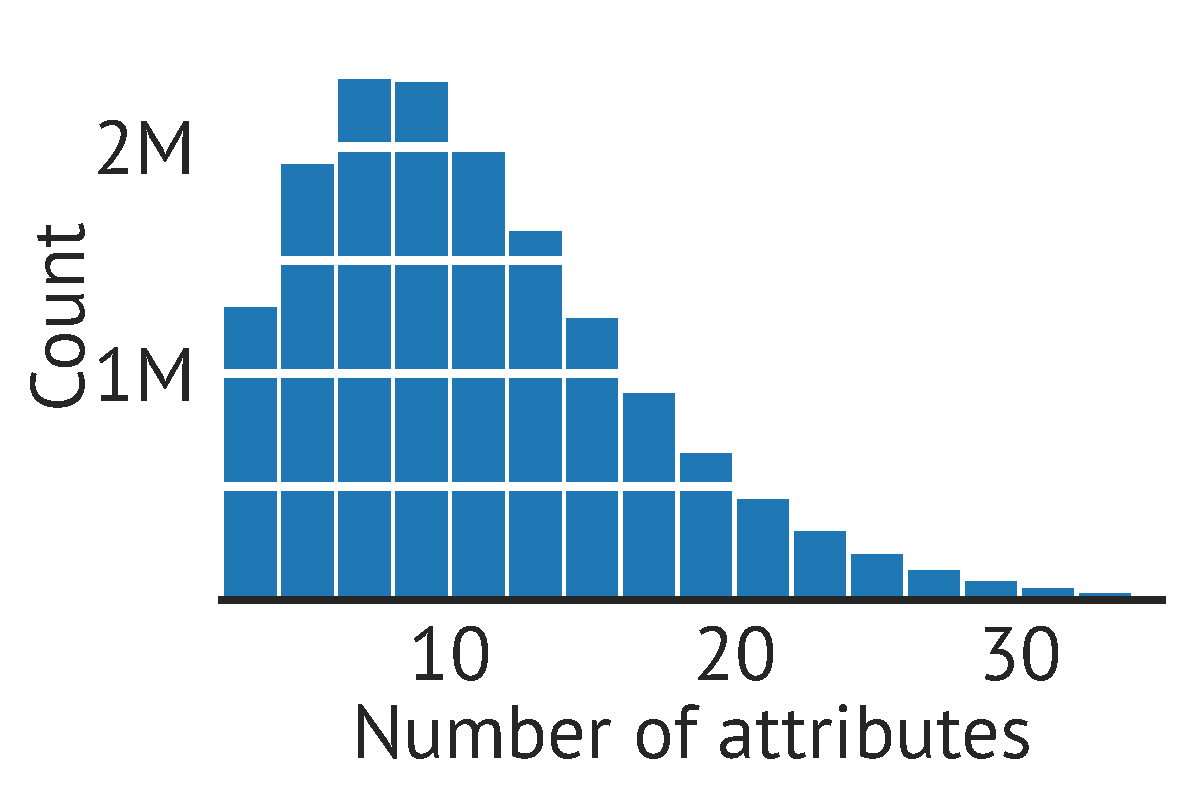
\includegraphics[width=0.6\linewidth]{fig/hist_meals}
%  \vspace*{-8mm}
  \caption{A histogram of the number of foods illustrates the statistical
    challenge of building models to rank from sets. Even in this subset of the
    data, 50k users consume 16M meals in one year. This means when building a
    model to rank meals, a model with unique parameters for every datapoint is
    inefficient: models should share parameters across meals.}
  % \end{minipage}
  % \begin{minipage}[c]{0.49\linewidth}
  %   \centering
  %   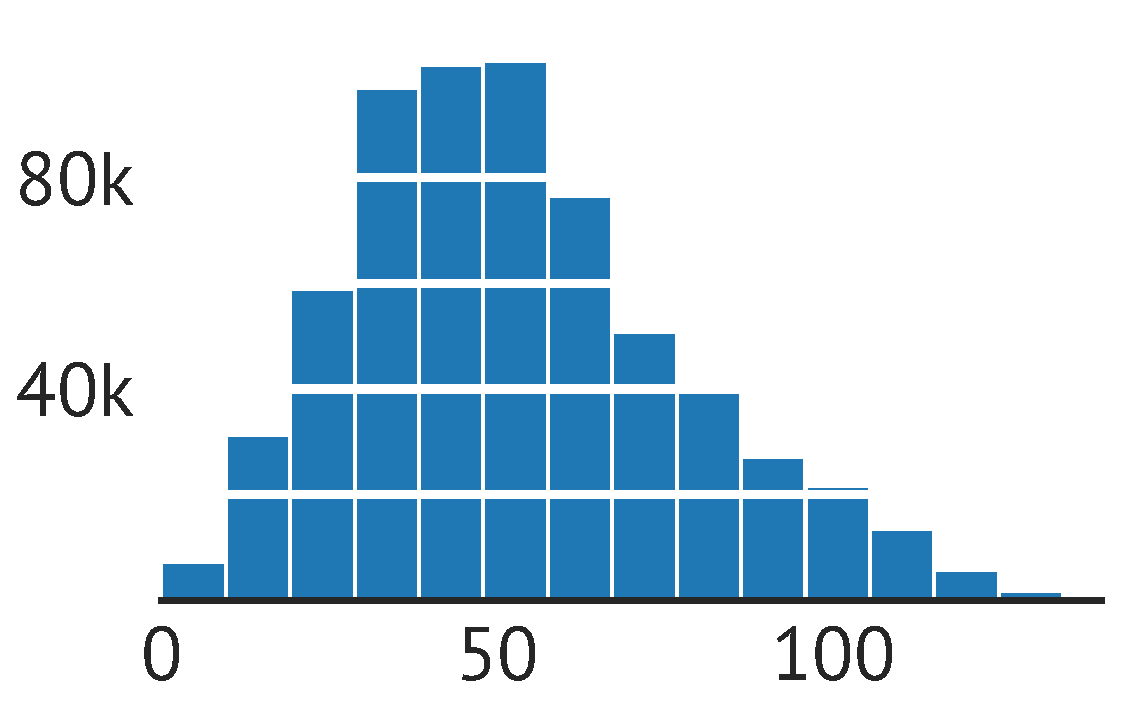
\includegraphics[width=\textwidth]{fig/hist_arxiv}
  %   \vspace*{-8mm}
  %   \caption*{\# words in arXiv abstracts}
  % \end{minipage}
  % \caption{\textbf{Corpora where items have set-valued attributes have a large
  %     number of unique features.}}
  \label{fig:hist}
\end{figure}


%%% Local Variables:
%%% mode: latex
%%% TeX-master: "../set_recommendation"
%%% End:


% % hook: why you should read on. world-as-it-could-be if you join us on the ride
% We develop \gls{rfs}, a recommendation model that meets the above
% criteria of parameter-sharing and order-invariance, and guarantees improvement
% in recall and ability to approximate other models. Other order-invariant models
% such as matrix factorization do not have such theoretical backing of improved
% evaluation metrics and ability to approximate other models. The theory we
% develop for \gls{rfs} frees practitioners to focus on building
% efficient architectures for one model, rather than comparing across that may not
% be able to approximate others, or that may not provably improve recall.

% % at a high level, what are the insights needed to solve the problem?
% The key insight that guarantees that \gls{rfs} improves recall is
% the framing of recall as classification. Recall measures the fraction of items a
% user consumed in a ranking returned by a recommendation model. This is
% inherently a binary task: a model does or does not recall an item. It follows
% that a perfect classifier maximizes recall. This framing enables us build
% \gls{rfs} as a classifier and leverage recent innovations from
% deep learning~\cite{Mikolov2013} to fit our model. We define negative samples as
% items users are unlikely to consume. This allows us to fit
% \gls{rfs} to implicit feedback data, where there are only
% user-item interactions, and users do not explicitly indicate dislike of items.

% % universal approximation
% The second goal of building a model that approximates others is achieved by
% parameterizing \gls{rfs} using neural networks. This enables us to
% show that the model can approximate other recommenders that rank from sets. We
% describe several neural network architectures, including one based on residual
% networks~\cite{DBLP:journals/corr/HeZRS15}.

% % !TEX root = ../set_recommendation.tex
\begin{figure*}[t!]
  \centering
%  \pdfimageresolution=500  
  \includegraphics[width=0.95\textwidth]{fig/arxiv_user_embeddings_tsne.png}
  \caption{\label{fig:arxiv_tsne} \acrlong{rfs} trained on arXiv reading
    behavior clusters researchers by their most frequently-read arXiv category
    (best viewed in color). On this data, \acrlong{rfs} is trained to recommend
    items using their attributes as described in \Cref{sec:experiments_arxiv};
    the set of attributes for a paper is the set of words in the abstract. A
    visualization of the user embeddings in the inner product regression
    function in \Cref{eqn:rankfromsets} yields an interpretable map of science.
    We use the t-SNE algorithm~\citep{maaten2008visualizing} for visualizing the
    high-dimensional embeddings in two dimensions. In this map of science,
    fields of study are related according to patterns in how people read papers
    in neighboring fields. Each marker represents a user embedding; the color
    assigned to a user is determined the user's most-read arXiv category. The
    color assigned to a category is determined by the most-read categories
    across the arXiv, with similar colors assigned to similar fields according
    to the arXiv ontology. For an interactive version of this map, please visit
    anon-url which enables zoom and display of all 143 arXiv category labels to
    explore the relationships between different fields of science.}
\end{figure*}


%%% Local Variables:
%%% mode: latex
%%% TeX-master: "../set_recommendation"
%%% End:


% % describe our model, how it is trained, an how it recommends
% \gls{rfs} is a classifier whose output is the probability of a
% user consuming an item. The model is trained to discriminate items users consume
% from items users are unlikely to consume (negative samples). The probability
% of item consumption output by the model is used to rank items for
% recommendation.

% % deep learning-> universal approximation, and architectures to satisfy
% % order-invariance and parameter-sharing
% We parameterize \gls{rfs} using neural networks, enabling the
% approximation of other models. The architectures of the neural networks are
% defined to meet the criteria of parameter-sharing and order-invariance arising
% from the properties of items represented by sets of attributes.

% % results
% We demonstrate our method by comparing it to several recommendation models on
% two datasets. The first dataset consists of users consuming $16$M meals from a
% food tracking app, and the second consists of users consuming $637$k preprints
% on the arXiv. The model outperforms order-invariant recurrent neural
% networks~\citep{Hochreiter1997}, a word embedding model~\citep{Mikolov2013}, and
% content-based Poisson factorization~\citep{Gopalana}. We also find that
% \gls{rfs} yields interpretable patterns in user behavior as in
% \Cref{fig:arxiv_tsne}.

% \paragraph{Related work.} Regression models such as deep
% sets~\citep{DBLP:journals/corr/ZaheerKRPSS17} have been developed for set-valued
% data. The deep sets model is a regression, not recommendation model, and does
% not use negative sampling in contrast to \gls{rfs}. Several
% recommendation algorithms use negative sampling to improve performance
% \cite{he2017neural,Chen:2017:SSN:3097983.3098202}. There are also deep learning
% models for collaborative filtering~\citep{zhang2017deep}. However, such work is
% centered on recommending items without side information. We focus on items with
% side information comprised of sets of attributes. In this regime the large
% number of unique sets of attributes is an obstacle and requires additional
% modeling choices. \citet{tansey2016diet2vec} also analyze diet data, but do not
% address recommendation. Probabilistic deep learning approaches for
% recommendation exist~\cite{Ranganath:2015} but do not include negative samples
% in the likelihood; we show this improves performance.

% % set up the task of recommendation, foreshadow how we will solve it via
% % classification
% Sets of attributes represent many types of items. A user might be associated
% with a photo that has tags, a disease with diagnosis codes, or a playlist of
% songs. Recommendation models for such items use the item attributes to rank
% items for users. Central to building recommendation models is evaluation, and a
% common metric is recall. But existing models such as matrix factorization do not
% have associated theoretical guarantees of improved recall. Currently, models are
% built on a case-by-case basis and adapted to the data at hand, and must be
% painstakingly compared to see which extension leads to improvement of the
% evaluation metric.

% % foreshadow desiderata
% Our goal is to build a recommendation model to rank items from attributes, and
% buttress the model with theoretical guarantees of universal approximation
% (ability to approximate other models) and of improved recommendation performance
% vis-\`a-vis recall.

% % desideratum #1: statistical challenge
% Building models that rank items from sets of attributes must address two
% difficulties arising from the properties of sets. The first difficulty is the
% statistical challenge posed by the large number of possible sets. The number of
% sets of attributes is large; we cannot posit a model with unique parameters for
% every set of attributes. The meal recommendation problem illustrates this
% statistical challenge. \Cref{fig:hist} shows the number of meals in data from a
% food tracking app. Even in this small fraction of the data, there are over ten
% million unique meals. In building a recommendation model to rank meals based on
% their constituent foods, the model should satisfy the criterion of
% parameter-sharing, and share parameters across meals with similar foods. For
% example, matrix factorization does not satisfy this criteria: it requires
% learning parameters for every meal. This is inefficient, as most meals are
% consumed by a single user in this data. The criterion of parameter-sharing is
% necessary for models to scale to large real-world datasets as in
% \Cref{fig:hist}.

% % desideratum #2
% In addition to parameter-sharing across sets, models that rank items based on
% their sets of attributes must be invariant to the order of set elements. This
% criterion is called order-invariance. For example, a meal is a set of foods, and
% remains the same meal if we permute the foods it contains. Recommendation models
% should yield the same output regardless of the order that set elements are fed
% to the model. Matrix factorization is an example of an order-invariant model.

% \begin{figure}[t!]
  \centering
  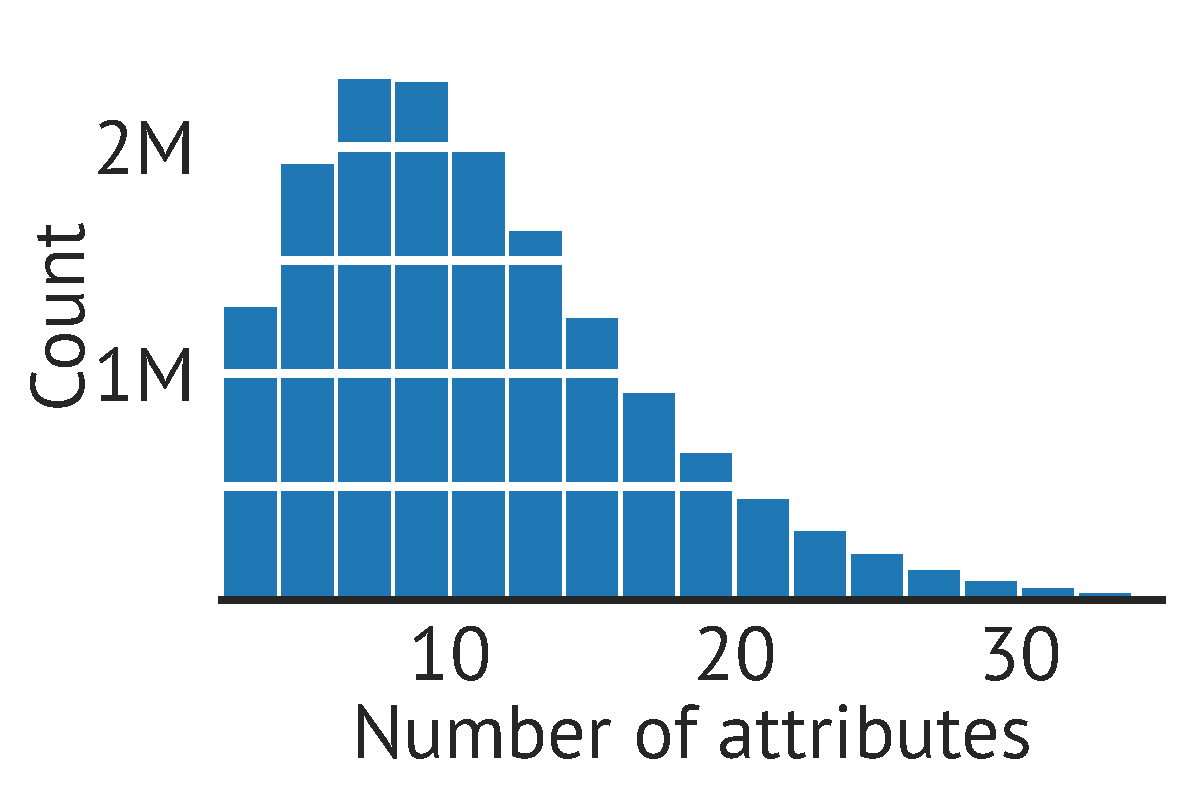
\includegraphics[width=0.6\linewidth]{fig/hist_meals}
%  \vspace*{-8mm}
  \caption{A histogram of the number of foods illustrates the statistical
    challenge of building models to rank from sets. Even in this subset of the
    data, 50k users consume 16M meals in one year. This means when building a
    model to rank meals, a model with unique parameters for every datapoint is
    inefficient: models should share parameters across meals.}
  % \end{minipage}
  % \begin{minipage}[c]{0.49\linewidth}
  %   \centering
  %   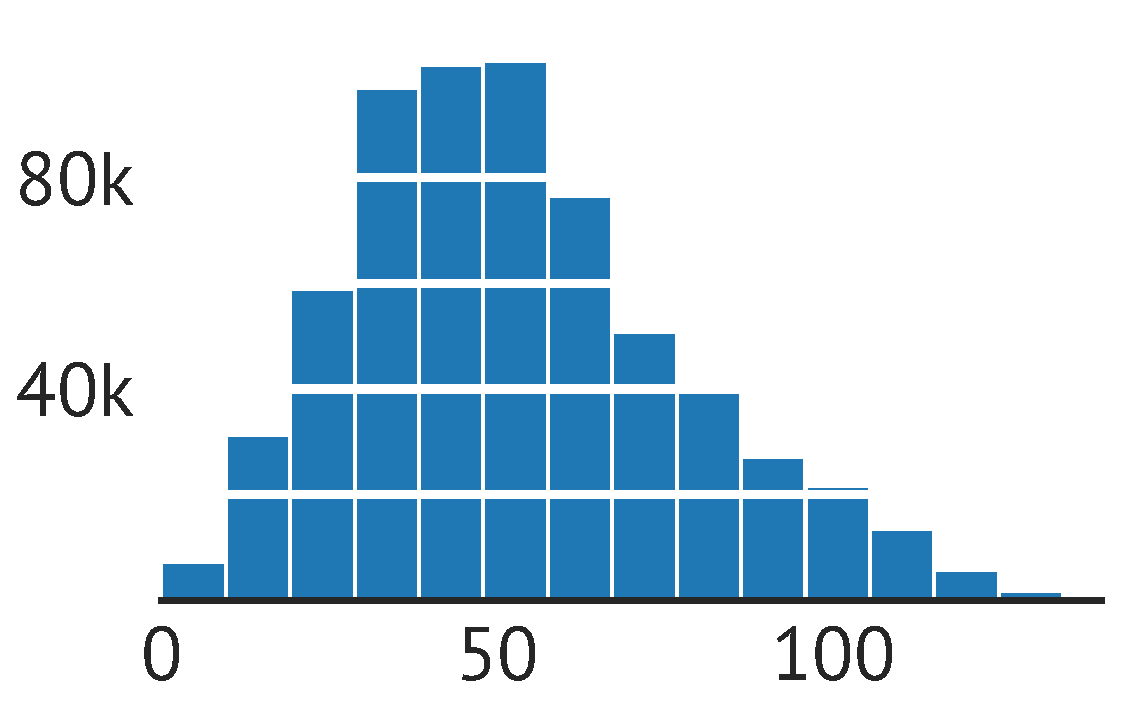
\includegraphics[width=\textwidth]{fig/hist_arxiv}
  %   \vspace*{-8mm}
  %   \caption*{\# words in arXiv abstracts}
  % \end{minipage}
  % \caption{\textbf{Corpora where items have set-valued attributes have a large
  %     number of unique features.}}
  \label{fig:hist}
\end{figure}


%%% Local Variables:
%%% mode: latex
%%% TeX-master: "../set_recommendation"
%%% End:


% % hook: why you should read on. world-as-it-could-be if you join us on the ride
% We develop \gls{rfs}, a recommendation model that meets the above
% criteria of parameter-sharing and order-invariance, and guarantees improvement
% in recall and ability to approximate other models. Other order-invariant models
% such as matrix factorization do not have such theoretical backing of improved
% evaluation metrics and ability to approximate other models. The theory we
% develop for \gls{rfs} frees practitioners to focus on building
% efficient architectures for one model, rather than comparing across models that
% may not provably improve recall (or be able to approximate other models).

% % at a high level, what are the insights needed to solve the problem?
% The key insight that guarantees that \gls{rfs} improves recall is
% the framing of recall as classification. Recall measures the fraction of items a
% user consumed in a ranking returned by a recommendation model. This is
% inherently a binary task: a model does or does not recall an item. It follows
% that a perfect classifier maximizes recall. This framing enables us build
% \gls{rfs} as a classifier and leverage recent innovations from
% deep learning~\cite{Mikolov2013} to fit our model. We define negative samples as
% items users are unlikely to consume. This allows us to fit
% \gls{rfs} to implicit feedback data, where there are only
% user-item interactions, and users do not explicitly indicate dislike of items.

% % universal approximation
% The second goal of building a model that approximates others is achieved by
% parameterizing \gls{rfs} using neural networks. This enables us to
% show that the model can approximate other recommenders that rank from sets. We
% describe several neural network architectures, including one based on residual
% networks~\cite{DBLP:journals/corr/HeZRS15}.

% % !TEX root = ../set_recommendation.tex
\begin{figure*}[t!]
  \centering
%  \pdfimageresolution=500  
  \includegraphics[width=0.95\textwidth]{fig/arxiv_user_embeddings_tsne.png}
  \caption{\label{fig:arxiv_tsne} \acrlong{rfs} trained on arXiv reading
    behavior clusters researchers by their most frequently-read arXiv category
    (best viewed in color). On this data, \acrlong{rfs} is trained to recommend
    items using their attributes as described in \Cref{sec:experiments_arxiv};
    the set of attributes for a paper is the set of words in the abstract. A
    visualization of the user embeddings in the inner product regression
    function in \Cref{eqn:rankfromsets} yields an interpretable map of science.
    We use the t-SNE algorithm~\citep{maaten2008visualizing} for visualizing the
    high-dimensional embeddings in two dimensions. In this map of science,
    fields of study are related according to patterns in how people read papers
    in neighboring fields. Each marker represents a user embedding; the color
    assigned to a user is determined the user's most-read arXiv category. The
    color assigned to a category is determined by the most-read categories
    across the arXiv, with similar colors assigned to similar fields according
    to the arXiv ontology. For an interactive version of this map, please visit
    anon-url which enables zoom and display of all 143 arXiv category labels to
    explore the relationships between different fields of science.}
\end{figure*}


%%% Local Variables:
%%% mode: latex
%%% TeX-master: "../set_recommendation"
%%% End:


% % describe our model, how it is trained, an how it recommends
% \gls{rfs} is a classifier whose output is the probability of a
% user consuming an item. The model is trained to discriminate items users consume
% from items users are unlikely to consume (negative samples). The probability
% of item consumption output by the model is used to rank items for
% recommendation.

% % deep learning-> universal approximation, and architectures to satisfy
% % order-invariance and parameter-sharing
% We parameterize \gls{rfs} using neural networks, enabling the
% approximation of other models. The architectures of the neural networks are
% defined to meet the criteria of parameter-sharing and order-invariance arising
% from the properties of items represented by sets of attributes.

% % results
% We demonstrate our method by comparing it to several recommendation models on
% two datasets. The first dataset consists of users consuming $16$M meals from a
% food tracking app, and the second consists of users consuming $637$k preprints
% on the arXiv. The model outperforms order-invariant recurrent neural
% networks~\citep{Hochreiter1997}, a word embedding model~\citep{Mikolov2013}, and
% content-based Poisson factorization~\citep{Gopalana}. We also find that
% \gls{rfs} yields interpretable patterns in user behavior as in
% \Cref{fig:arxiv_tsne}.

% \paragraph{Related work.} Regression models such as deep
% sets~\citep{DBLP:journals/corr/ZaheerKRPSS17} have been developed for set-valued
% data. The deep sets model is a regression, not recommendation model, and does
% not use negative sampling in contrast to \gls{rfs}. Several
% recommendation algorithms use negative sampling to improve performance
% \cite{he2017neural,Chen:2017:SSN:3097983.3098202}. There are also deep learning
% models for collaborative filtering~\citep{zhang2017deep}. However, such work is
% centered on recommending items without side information. We focus on items with
% side information comprised of sets of attributes. In this regime the large
% number of unique sets of attributes is an obstacle and requires additional
% modeling choices. \citet{tansey2016diet2vec} also analyze diet data, but do not
% address recommendation. Probabilistic deep learning approaches for
% recommendation exist~\cite{Ranganath:2015} but do not include negative samples
% in the likelihood; we show this improves performance.

%%% Local Variables:
%%% mode: latex
%%% TeX-master: "set_recommendation"
%%% End: